\chapter{Modelowanie procesu}
	\label{ch:mod}
	
	\section{Opóźnienie}
		\label{sec:tau}
		
		W celu zdefiniowania opóźnienia $\tau$ procesu zasymulowaliśmy go dla pojedynczego skoku sterowania. Wyniki symulacji przedstawione są na wykresie \ref{fig:tau}. Skok sterowania nastąpił w 5 kroku działania programu, natomiast wyjście procesu zmieniło się dopiero w kroku 8. Oznacza to, że poszukiwane przez nas opóźnienie wynosi $\tau = 3$. Użyty przez nas skrypt to $tauwiz.m$.
		
		\begin{figure}[h!]
			\centering
			\includegraphics[width=\linewidth]{img/tau_wizualizacja.eps}
			\caption{Wizualizacja opóźnienia procesu}
			\label{fig:tau}
		\end{figure}
	
	\newpage
	\section{Dobór liczby neuronów}
		\label{sec:neurony}
		
		W celu dobrania odpowiedniej liczby neuronów dla sieci zastosowaliśmy wielokrotne uczenie z użyciem programu $sieci.exe$. Dla każdej ilości neuronów ukrytych od 1 do 10 dokonaliśmy 5 procesów uczenia za pomocą algorytmu BFGS z wykorzystaniem rekurencji. W tym celu wykorzystaliśmy skrypt $modelowanie.m$. Najmniejszy uzyskany błąd uczenia wraz ze skojarzonym z nim błędem weryfikacji przedstawiony został w tabeli poniżej. Najmniejszy błąd dla obydwu zbiorów występuje dla 9 neuronów. Ostatecznie jednak zdecydowaliśmy się na używanie sieci z pięcioma neuronami ukrytymi. Powodem tego jest mała poprawa w stosunku do większych ilości neuronów oraz chęć zmniejszenia nakładu obliczeń. Dodatkowo sieci o zbyt dużej ilości neuronów ukrytych mają tendencję do przetrenowywania się, w wyniku którego sieć przystosowuje się nie tyle do procesu co do samych danych uczących.
		
		\begin{table}[h!]
			\centering
			\begin{tabular}{c|l|l}
				Liczba neuronów&Błąd uczenia&Błąd weryfikacji\\\hline
				1&3.070626e+01&5.548815e+01\\\hline
				2&4.977413e-01&1.060318e+00\\\hline
				3&3.206039e-01&5.111444e-01\\\hline
				4&1.479096e-01&2.625729e-01\\\hline
				5&8.734595e-02&1.534512e-01\\\hline
				6&7.765994e-02&2.087909e-01\\\hline
				7&2.614618e-02&1.727668e-01\\\hline
				8&1.509561e-02&1.095385e-01\\\hline
				9&1.355132e-02&6.725641e-02\\\hline
				10&2.105601e-02&1.136051e-01\\\hline
			\end{tabular}
		\caption{Błędy modelu dla różnej ilości neuronów}
		\label{tab:neurony}
		\end{table}
		
		\newpage
	\section{Model z algorytmu BFGS}
		\label{sec:bfgs}
		Na wykresie \ref{fig:bfgs_oe_p} przedstawione zostały błędy predykatorów ARX i OE dla kolejnych iteracji uczenia modelu. Zgodnie z ustaleniami z poprzednich punktów zastosowane zostały następujące parametry: $tau = 3$, $neurony$ $ukryte = 5$. Końcowe błędy dla obydwu predykatorów wynosiły odpowiednio: $Eoe = 0.0787$ i $Earx = 0.0212$. Jak widać błędy te są dosyć małe jak na 2000 próbek co oznacza, że sieć dobrze nauczyła się modelu.
		
		\begin{figure}[h!]
			\centering
			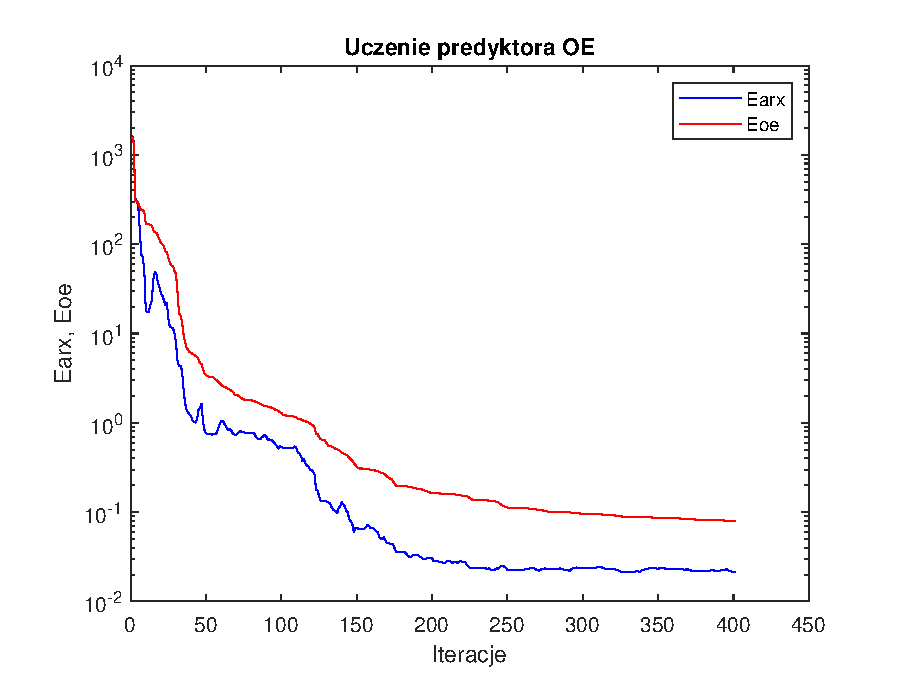
\includegraphics[width=\linewidth]{img/BFGS_OE_p.eps}
			\caption{Zmiany błędów predykatora ARX i OE dla kolejnych iteracji uczenia modelu algorytmem BFGS z użyciem rekurencji}
			\label{fig:bfgs_oe_p}
		\end{figure}
		
		\newpage
	\section{Symulacja modelu z algorytmu BFGS}
		\label{sec:bfgs_sym}
		Model z poprzedniego punktu został zasymulowany w trybie rekurencyjnym dla uczącego oraz weryfikującego zbioru danych. Błędy dla obydwu zbiorów danych wyniosły odpowiednio: $Eucz = 0.0787$ oraz $Ewer = 0.2172$. Błedy otrzymywane były ze wzoru:
		\begin{equation}
		\begin{tabular}{l}
		$E = (y(S:end)-y^M(S:end))'*(y(S:end)-y^M(S:end))$
		\end{tabular}
		\label{eq:error}
		\end{equation}
		gdzie $S = max(n_A,n_B)+1$, oraz $n_A$ i $n_B$ są współczynniki modelu opisanego wzorem
		\begin{equation}
		\begin{tabular}{l}
		$\hat{y}(k)=f(u(k-\tau),...,u(k-n_B),y(k-1),...,y(k-n_A))$
		\end{tabular}
		\label{eq:model_wzor}
		\end{equation}
		
		\begin{figure}[h!]
			\centering
			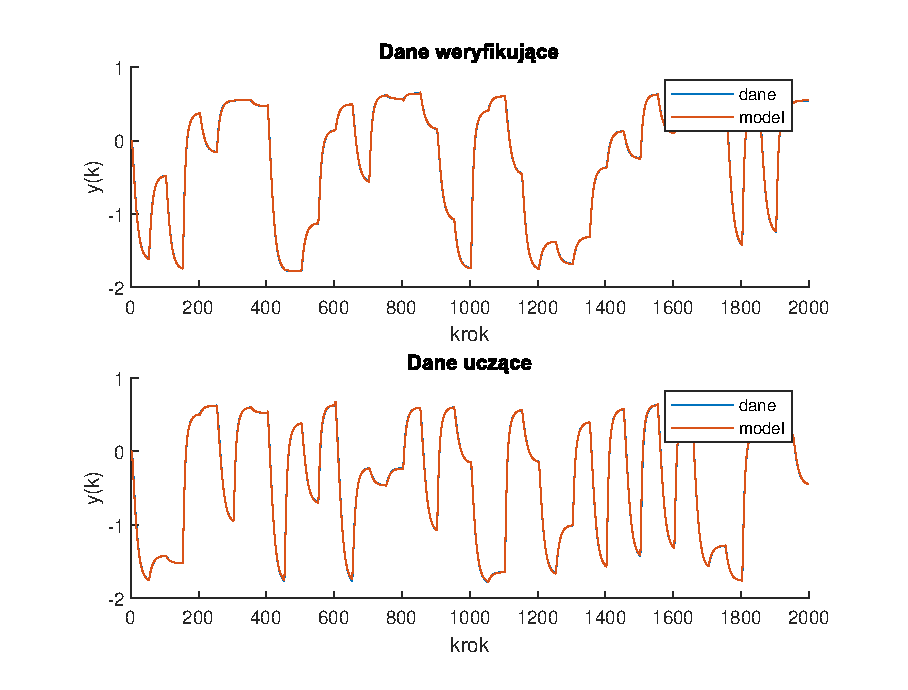
\includegraphics[width=\linewidth]{img/BFGS_OE_d.eps}
			\caption{Symulacja modelu uczonego algorytmem BFGS z rekurencją na danych uczących i weryfikujących}
			\label{fig:bfgs_oe_d}
		\end{figure}
		
		\newpage
	\section{Model z algorytmu najszybszego spadku}
		\label{sec:naj_sp}
		Jak widać po poniższych wartościach błędów uczenia oraz z wykresu \ref{fig:ns_oe_p} algorytm najszybszego spadku nie radzi sobie najlepiej z uczeniem sieci co skutkuje dużą niedokładnością modelu. Końcowe błędy dla obydwu predykatorów wyniosły $Eoe = 25.1864$ oraz $Earx = 1.7730$, co w obydwu przypadkach wynosi więcej niż przy uczeniu sieci metodą BFGS.
		
		\begin{figure}[h!]
			\centering
			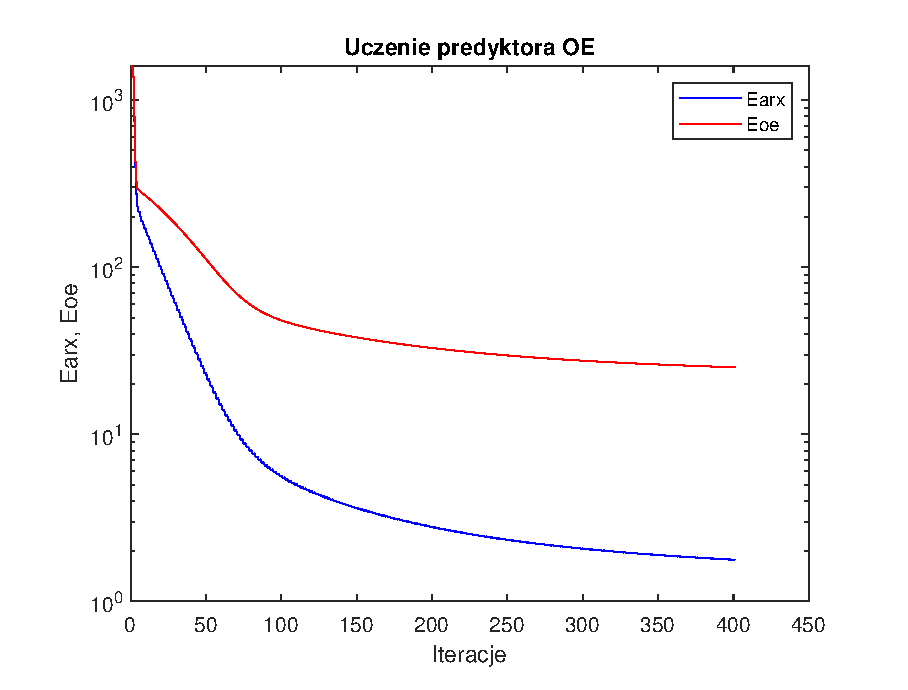
\includegraphics[width=\linewidth]{img/NS_OE_p.eps}
			\caption{Zmiany błędów predykatora ARX i OE dla kolejnych iteracji uczenia modelu algorytmem najszybszego spadku z użyciem rekurencji}
			\label{fig:ns_oe_p}
		\end{figure}
		
		\newpage
	\section{Model z algorytmu BFGS z uczeniem bez rekurencji}
		\label{sec:bfgs_arx}
		Na wykresie \ref{fig:bfgs_arx_p} można zobaczyć, że algorytm BFGS w wersji bez rekurencji radzi sobie niewiele gorzej niż algorytm BFGS w wersji z rekurencją. Po kilku próbach uczenia sieci udało się osiągnąć błędy uczenia o wartościach Eoe = 0.0925 i Earx = 0.0237, co nadal jest bardzo dobrym wynikiem.
		
		\begin{figure}[h!]
			\centering
			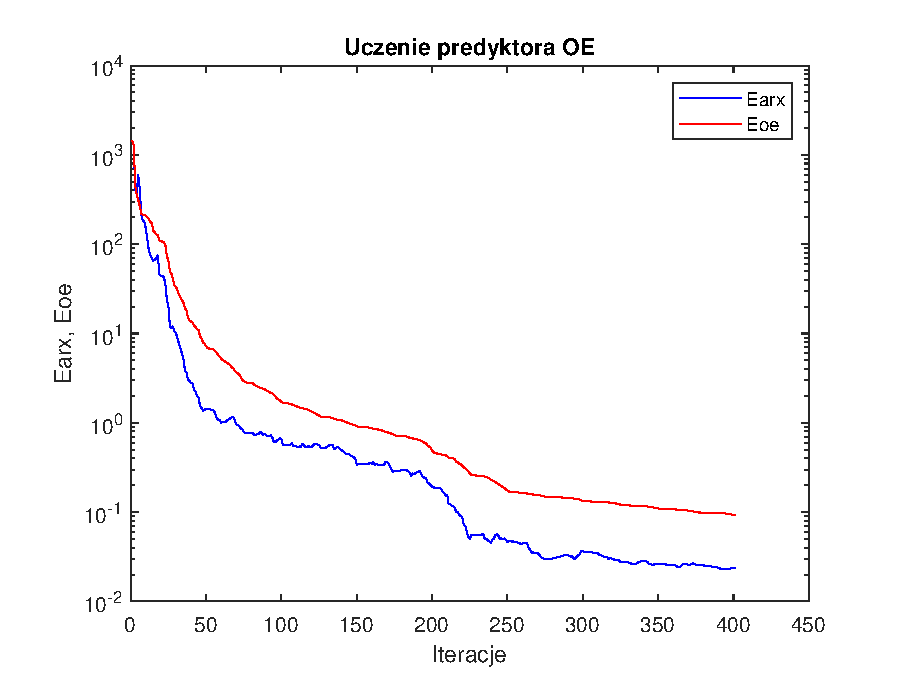
\includegraphics[width=\linewidth]{img/BFGS_ARX_p.eps}
			\caption{Zmiany błędów predykatora ARX i OE dla kolejnych iteracji uczenia modelu algorytmem BFGS bez użycia rekurencji}
			\label{fig:bfgs_arx_p}
		\end{figure}
		
		\newpage
	\section{Symulacja modelu z algorytmu BFGS z uczeniem bez rekurencji}
		\label{sec:bfgs_arx_sym}
		Podobnie jak w przypadku modelu nauczonego algorytmem z rekurencją, model z poprzedniego punktu został zasymulowany w trybie rekurencyjnym dla uczącego oraz weryfikującego zbioru danych. Błędy dla obydwu zbiorów danych wyniosły odpowiednio: Eucz = 0.0925 oraz Ewer = 0.3542. Mimo niewielkiej różnicy model ten sprawuje się niestety gorzej niż w wersji z rekurencją, dlatego to na tamtym będziemy wykonywać następne zadania. Jest to logiczne, gdyż model symulowany jest w trybie rekurencyjnym, a uczony był bez niej, więc z oczywistych powodów powinien być gorszy niż model uczony z rekurencją.
		
		\begin{figure}[h!]
			\centering
			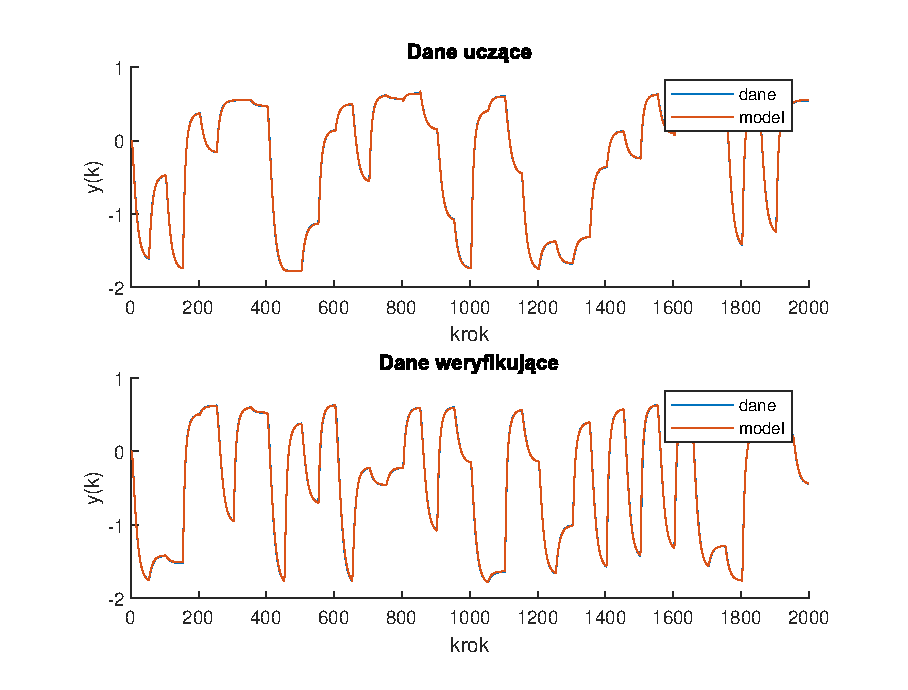
\includegraphics[width=\linewidth]{img/BFGS_ARX_d.eps}
			\caption{Symulacja modelu uczonego algorytmem BFGS bez rekurencji na danych uczących i weryfikujących}
			\label{fig:bfgs_arx_d}
		\end{figure}
		
		\newpage
	\section{Model metodą najmniejszych kwadratów}
		\label{sec:mnk}
		Uczenie modelu metodą najmniejszych kwadratów relizowane jest za pomocą obecnej w Matlabie operacji lewego dzielenia:
		\begin{equation}
		\begin{tabular}{l}
		$w = $ $\begin{bmatrix}b_3\\b_4\\a_1\\a_2\end{bmatrix}$ $=M\backslash y_{ucz}(5:end)$
		\end{tabular}
		\label{eq:mnk}
		\end{equation}
		gdzie
		\begin{equation}
		\begin{tabular}{l}
		$M = $ $\begin{bmatrix}x_{ucz}(2)&x_{ucz}(1)&y_{ucz}(4)&y_{ucz}(3)\\.&.&.&.\\.&.&.&.\\.&.&.&.\\x_{ucz}(n-\tau)&x_{ucz}(n-\tau -1)&y_{ucz}(n-1)&y_{ucz}(n-2)\end{bmatrix}$
		\end{tabular}
		\label{eq:M_mnk}
		\end{equation}
		oraz $n =$ liczba próbek.
		
		Otrzymane błędy były równe: $Ewer = 294.6949$ oraz $Eucz = 299.7408$. Jak widać jakość tego modelu jest bardzo zła i błędy są większe, niż w przypadku modelu uczonego algorytmem BFGS lub najszybszego spadku. Przebiegi przedstawiające działanie modelu dla danych uczących i weryfikujących pokazane są poniżej. Do wyznaczenia modelu oraz wyrysowania wykresu użyty został skrypt $mnk.m$.
		
		\begin{figure}[h!]
			\centering
			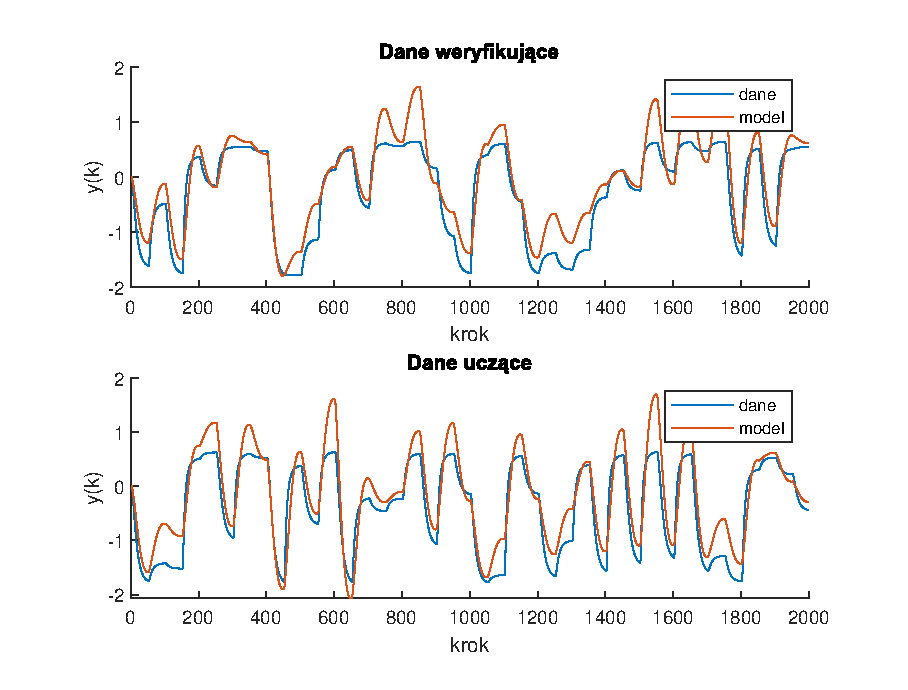
\includegraphics[width=\linewidth]{img/mnk.eps}
			\caption{Symulacja modelu wykonanego za pomocą metody najmniejszych kwadratów}
			\label{fig:mnk}
		\end{figure}